\documentclass[12pt]{article}
\usepackage{algorithm}
\usepackage{geometry}             
\usepackage{moreverb}   
\usepackage{longtable}
\usepackage{fancyhdr}
\geometry{letterpaper}
\usepackage{algorithmic}             
\usepackage{algorithm}
\usepackage{array}     
\usepackage{hyperref}
\usepackage{graphicx}
\usepackage{subfigure}
\usepackage{fullpage}
\usepackage{amsmath, amssymb, amsthm}
\usepackage[framed,numbered,autolinebreaks,useliterate]{mcode}
\usepackage{mathabx}
\usepackage{float}

\newtheorem{theorem}{Theorem}
\newtheorem{corollary}{Corollary}
\newtheorem{proposition}{Proposition}
\newtheorem{lemma}{Lemma}
\newtheorem{definition}{Definition}
\newtheorem{remark}{Remark}
\newtheorem{notation}{Notation}

% my macros
\newcommand{\paren}[1]{\left({#1}\right)}
\newcommand{\bracket}[1]{\left[{#1}\right]}
\newcommand{\curly}[1]{\left\{{#1}\right\}}
\newcommand{\vecb}[1]{\mathbf{#1}}
\newcommand{\matb}[1]{\mathbf{#1}}
\newcommand{\V}[1]{\mathbf{#1}}
\newcommand{\m}[1]{\mathbf{#1}}
\newcommand{\inhomog}[1]{\widetilde{#1}}
\newcommand{\transpose}[1]{{#1}^\top}

\begin{document}

\title{CS 283 Final Project \\ Pipeline for Improving Accuracy of Hand Tracking with a Poorly Trained Haar Cascade Detector}
\date{Fall 2012}
\author{Kenny Yu (\href{mailto:kennyyu@college.harvard.edu}{kennyyu@college.harvard.edu})}
\maketitle

%%%%%%%%%%%%%%%%%%%%%%%%%%%%%%%%%%%%%%%%%%%%%%%%%%%%%
\section{Introduction}
What if you had the power of Microsoft's Kinect in your webcam? What if you could control applications simply with a swipe of your hand? Detecting and tracking hands typically requires a good detector, which requires large amounts of good data (usually at least 5000 images \cite{cascadetutorial}) and a tremendous amount of computation time to train the classifier. In this paper, we trained our hand detector with only 250 images, generated from 10 positives and 100 negatives. Despite this poorly trained Haar cascade classifier \cite{violajones}, we provide a pipeline to improve accuracy during hand tracking, achieving comparable results to tracking with a well-trained hand detector. Using this pipeline, we create a sample application \ref{mapsapp} in which the user can control Google Maps \cite{googlemaps} by simply moving one's hand. See our source code in \ref{sourcecode} or our pipeline and server to run this application.

\section{Methods}

\subsection{Training the Hand Detector}
To generate our hand detector, we took 10 pictures of our right hand using a webcam from a  Macbook Pro 2011 model, and we cropped the images to leave only our hand in the images. Our pictures consisted of our right hand with the palm facing forward and all fingers together. See Figure \ref{traininghands} for the the images we used as positives. We used the first 100 images from \cite{negatives} as negatives. We used OpenCV's \texttt{opencv\_createsamples} \cite{cascadetutorial}utility to generate 250 90 $\times$ 50 pixel samples from this set of 10 positives and 100 negatives, resulting in images where our positive images have been warped by homographies and placed randomly into our negative images. We used OpenCV's \texttt{opencv\_haartraining} tool to train our Haar cascade classifier, setting our min hit rate to $0.999$, our max false alarm rate to $0.5$, and running 14 stages in our cascade. This took about a day to complete, and the resulting cascade is located in \texttt{cascades/hand\_front.xml}.

\noindent\begin{figure}[H]
\centering
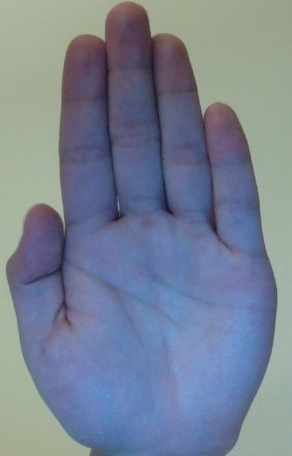
\includegraphics[width=50px, height=90px]{../data/positives/img0000.jpg}
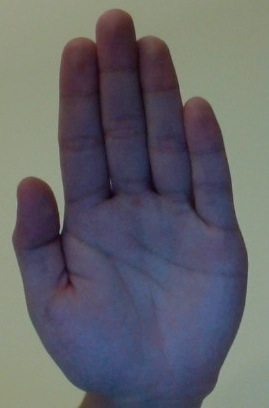
\includegraphics[width=50px, height=90px]{../data/positives/img0001.jpg}
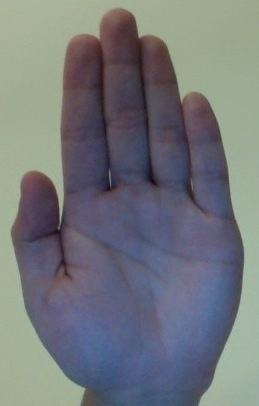
\includegraphics[width=50px, height=90px]{../data/positives/img0002.jpg}
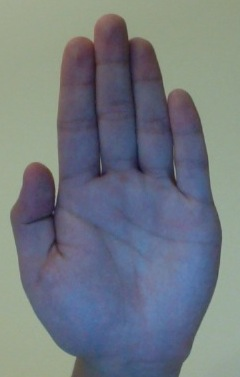
\includegraphics[width=50px, height=90px]{../data/positives/img0003.jpg}
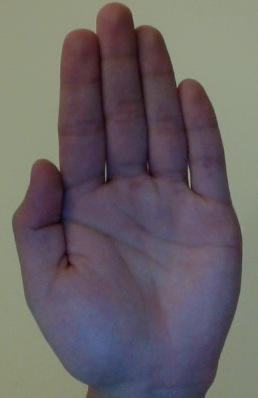
\includegraphics[width=50px, height=90px]{../data/positives/img0004.jpg} \\
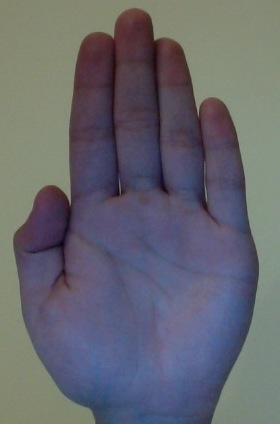
\includegraphics[width=50px, height=90px]{../data/positives/img0005.jpg}
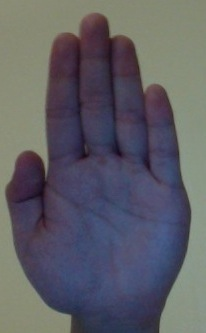
\includegraphics[width=50px, height=90px]{../data/positives/img0006.jpg}
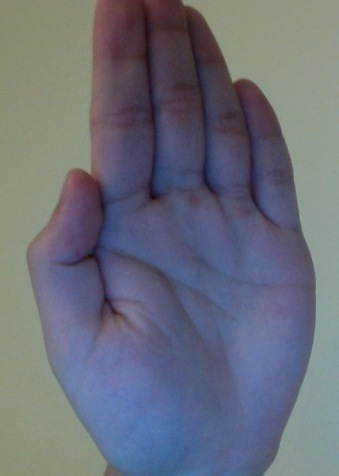
\includegraphics[width=50px, height=90px]{../data/positives/img0007.jpg}
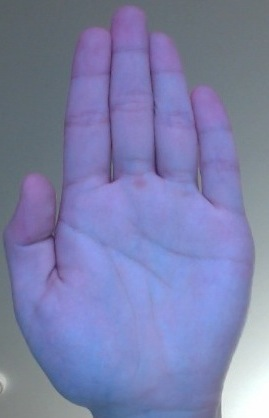
\includegraphics[width=50px, height=90px]{../data/positives/img0008.jpg}
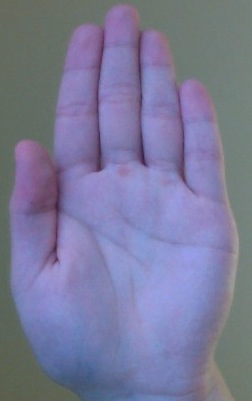
\includegraphics[width=50px, height=90px]{../data/positives/img0009.jpg}
\caption{The 10 positive images used to train our hand detector. We generated 250 samples from these, each of size 90 pixels high and 50 pixels wide.}
\label{traininghands}
\end{figure}

\subsection{Building the Pipeline}

See \texttt{detect.py} for the different components of our pipeline, and see \texttt{pipeline.py} for the various pipelines. For our pipeline, we used a frame size of 320 pixels wide and 240 pixels tall. We ran our detector without any preprocessing, and noted that we had many noisy detections, as shown in Figure \ref{1-original}. The yellow boxes indicate multiple possible detected hands, and the green one represents the largest one in the overall frame. We noted that our detector often mistook faces as hands, probably because of similar color tone. Using this heuristic, we decided to remove faces, and this generally gave us better results, as shown in \ref{2-noface}. We used OpenCV's frontal face detector in \texttt{cascades/haarcasacade\_frontalface\_alt.xml}, which works very well in practice.

Next, we noted that our detection was sensitive to noisy non-solid backgrounds. To account for this, we implemented background subtraction. To do this, we kept a history of the past $n$ frames, and we took the difference of the intensities of each pixel in the current frame and the oldest of the $n$ frames, and thresholded the difference. We found that setting our threshold to $20$ worked best, and we found that the number of frames $n = 20$ worked quite well. See Figure \ref{3-nobg} to see an example of the result of applying background subtraction. Background subtraction, however, had several issues. The dark patches left in the middle of the hand would sometimes prevent valid detections, and the randomly scattered dark patches also led to some false positive detections. 

To fix the latter issue, we used a simplified version of a Kalman Filter \cite{kalmanfilter} to predict a bounding box window of where the hand would likely be in the next frame. We made the assumption that a hand typically moves in a smooth manner, and so using the velocity and current position of the hand will give us a pretty good prediction for where the hand will be in the next frame. 

We defined our state $\m{x_k}$ at step $k$ to be a 4-vector:
$$\m{x_k} = \transpose{(x, y, v_x, v_y)},$$
where $x,y$ is the current position (center) of the hand, and $v_x, v_y$ are the $x$ and $y$ components of the velocity of the hand. From this definition of our state, we naturally defined the next state (prediction) $\m{x_{k+1}}$ to be:
$$\m{x_{k+1}} = \transpose{(x + v_x, y + v_y, v_x, v_y)},$$
where we obtained the new $x,y$ components by adding the corresponding components in the velocity. Thus, our transition matrix $\m{A}$ satisfies the equation
$$\m{x_{k+1}} = \m{A} \m{x_k},$$
where
$$\m{A} = 
\begin{bmatrix}
1 & 0 & 1 & 0 \\
0 & 1 & 0 & 1 \\
0 & 0 & 1 & 0 \\
0 & 0 & 0 & 1
\end{bmatrix}.
$$
When we first attempted to use this Kalman filter, we had used error, process noise, and measurement noise covariance matrices, however, we discovered that reducing the Kalman filter to a simple Markov process improved runtime performance and greatly simplified the overall model. 

In our pipeline, we used our Kalman filter to predict a state $\m{x_{k+1}} = (x,y,v_x,v_y)$, where $(x,y)$ represents our prediction of the center of a $h \times w$ bounding box where we would probably detect our hand. In practice, we discovered that a $h = 180, w = 100$ worked best. Given this window, we applied our hand detector only within this window. See Figure \ref{4-kalman} for the result of this hand detection, and see the blue box in Figure \ref{5-optical} to see the Kalman prediction window relative to the original frame. 

We detected the corners within the detected hand, and then we used Lucas-Kanade \cite{lucaskanade} to compute the optical flow of these corners. We summed the overall displacements to obtain the overall velocity $(\hat{v_x}, \hat{{v_y}})$. To correct our estimate, we set our corrected state $\m{\hat{x_k}}$ to be:
$$\m{\hat{x_k}} = \transpose{(\hat{x}, \hat{y}, c\hat{v_x}, c\hat{v_y})},$$
where $(\hat{x},\hat{y})$ is the center of the detected hand, and $c$ is constant we chose to scale back the overall direction. If $c$ is too large, then our window will overshoot the position of the hand. If $c$ is too small, then our hand will move past the prediction window and will not be detected. In practice, we discovered that $c = 0.02$ works best. We then obtained our prediction $\m{x_{k+1}}$ for the next frame by using our corrected state $\m{\hat{x_k}}$:
$$\m{x_{k+1}} = \m{A} \m{\hat{x_k}}.$$
When there are no detected hands, we set our Kalman prediction to be the entire original frame. Our final pipeline is listed in Algorithm \ref{pipeline}.



\noindent\begin{figure}[H]
\centering
\subfigure[Our hand classifier had many noisy detections.]{
	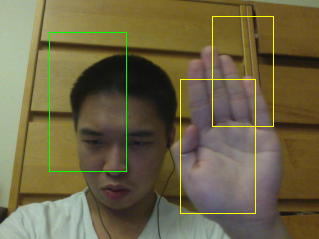
\includegraphics[width=220px, height=165px]{1-original.png}
	\label{1-original}
}
\subfigure[Face Removal]{
	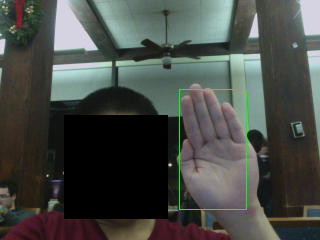
\includegraphics[width=220px, height=165px]{2-noface.png}
	\label{2-noface}
}
\subfigure[Background Subtraction]{
	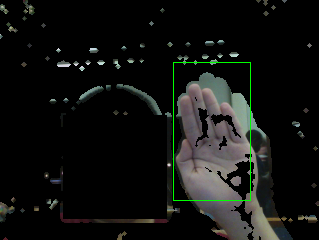
\includegraphics[width=220px, height=165px]{3-nobg.png}
	\label{3-nobg}
}
\subfigure[Kalman Prediction Window]{
	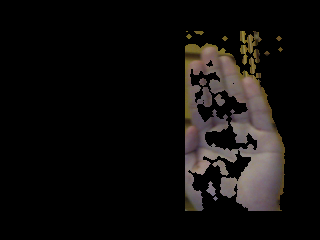
\includegraphics[width=220px, height=165px]{4-kalman.png}
	\label{4-kalman}
}
\subfigure[Final Detection and Optical Flow]{
	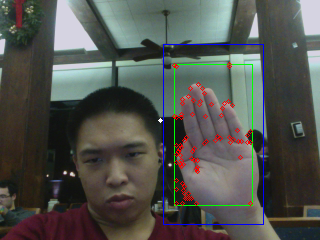
\includegraphics[width=220px, height=165px]{5-optical.png}
	\label{5-optical}
}
\caption{Our pipeline and hand detections at each stage. Green box - largest detected hand. Yellow boxes - other detections. Blue box - Kalman filter prediction. Red dots - corners.}
\label{all}
\end{figure}

\begin{algorithm}
\caption{Pipeline for Improving Accuracy of Hand Tracking with a Poorly Trained Hand Detector.}
\label{pipeline}

\noindent Given the current frame and the next frame:
\begin{enumerate}
\item {\bf Face Removal.} Apply OpenCV's frontal face detector and remove all detected faces.
\item {\bf Background Subtraction.} Eliminate the background by subtracting the intensities in the current frame and previous $n$-th frame, and threshold the difference.
\item {\bf Kalman Prediction.} Use our simplified Kalman filter to predict the likely bounding box of the hand in the current frame. If the previous frame had no detected hand, then our Kalman filter will estimate the entire frame as the bounding box.
\item {\bf Hand Detection.} Apply our hand detector within the bounding box (blue box) predicted by our Kalman Filter. If there are multiple detections (yellow boxes), take the first hand with the largest bounding box (green box)
\item {\bf Corner Detection.} If there are no detections, then output $(0,0)$ as our velocity. If there is a detection, compute the corners (red points) within the bounding box of our hand.
\item {\bf Optical Flow.} Use Lucas-Kanade to compute the optical flow of the detected corners, finding the corresponding points (if they exist) in the subsequent frame. Sum all the vector displacements (green vectors) to compute the overall velocity of the hand (white vector).
\item {\bf Kalman Update.} Update our Kalman Filter with the measured position and velocity of our detected hand, and repeat on the next frame.
\end{enumerate}
\end{algorithm}

\subsection{Building the Google Maps Application}

We used our pipeline to create a simple application in which the user can control Google Maps by moving one's hand. We follow the model proposed in \cite{webtutorial} to create our application. We used Chrome's WebRTC \cite{webrtc} ability to capture a video stream from a connected webcam. Using web sockets \cite{websockets}, we send a constant stream of frames to our server that is running our pipeline. We used Tornado 2.4.1 \cite{tornado} to run our server, and we used OpenCV 2.4.1\cite{opencv} to implement our pipeline. The server runs the pipeline and outputs the annotated frame and the overall computed direction of the hand, and the client then uses this information to update the map accordingly. A live running instance of the application can be publicly accessed at \url{http://goo.gl/pcNxG}. We set up this server on a medium Amazon EC2 instance. See Figure \ref{map} for a screenshot of the application in action. The green vectors represents the direction of the corners, and the white vector is the sum of the green vectors, representing the overall direction of the hand.

\noindent\begin{figure}[H]
\centering
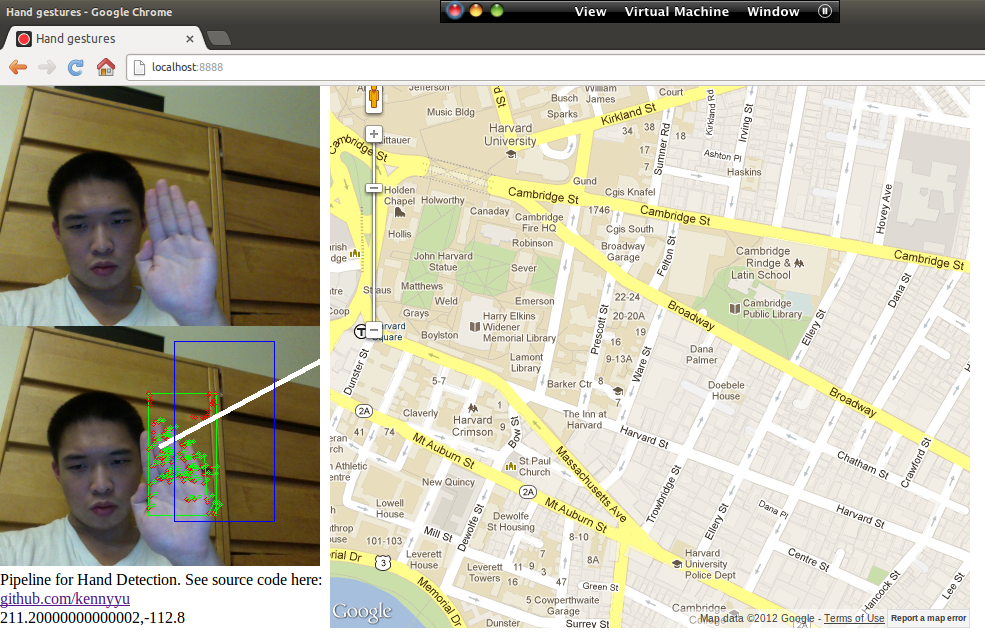
\includegraphics[scale=0.45]{map.png}
\caption{Screenshot of our Google Maps Application in action. The green vectors represents the direction of the corners, and the white vector is the sum of the green vectors, representing the overall direction of the hand.}
\label{map}
\end{figure}

\section{Results}

\noindent\begin{figure}[H]
\centering
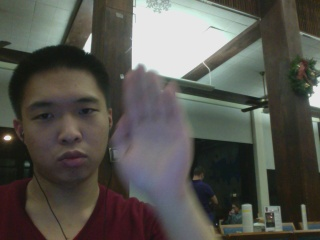
\includegraphics[width=40px, height=30px]{../data/analysis/img0000.jpg}
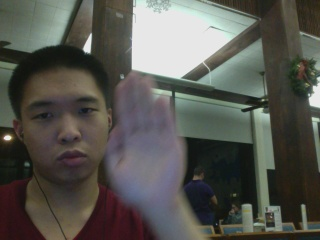
\includegraphics[width=40px, height=30px]{../data/analysis/img0001.jpg}
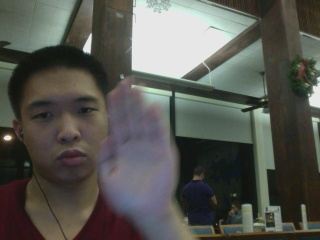
\includegraphics[width=40px, height=30px]{../data/analysis/img0002.jpg}
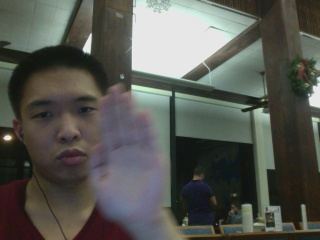
\includegraphics[width=40px, height=30px]{../data/analysis/img0003.jpg}
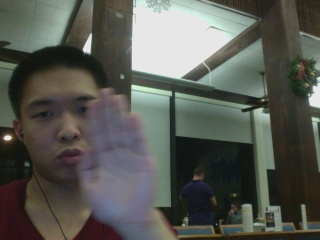
\includegraphics[width=40px, height=30px]{../data/analysis/img0004.jpg}
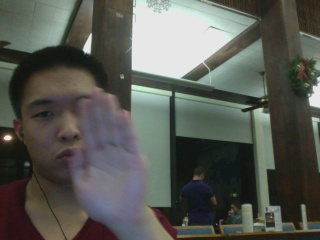
\includegraphics[width=40px, height=30px]{../data/analysis/img0005.jpg}
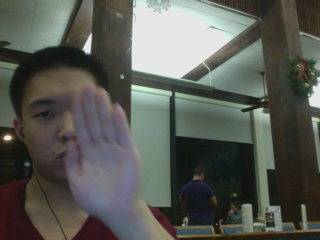
\includegraphics[width=40px, height=30px]{../data/analysis/img0006.jpg}
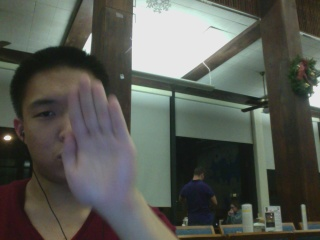
\includegraphics[width=40px, height=30px]{../data/analysis/img0007.jpg}
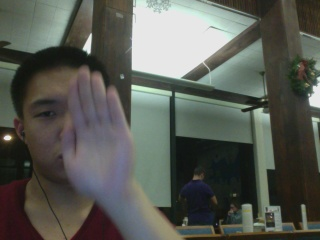
\includegraphics[width=40px, height=30px]{../data/analysis/img0008.jpg}
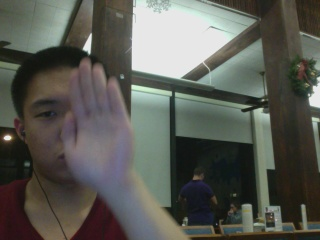
\includegraphics[width=40px, height=30px]{../data/analysis/img0009.jpg} \\
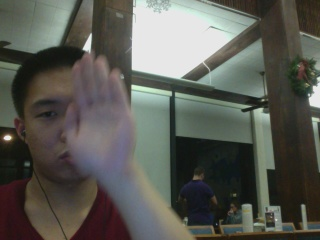
\includegraphics[width=40px, height=30px]{../data/analysis/img0010.jpg}
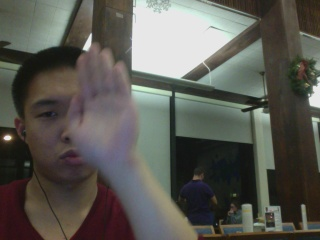
\includegraphics[width=40px, height=30px]{../data/analysis/img0011.jpg}
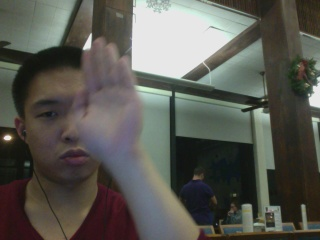
\includegraphics[width=40px, height=30px]{../data/analysis/img0012.jpg}
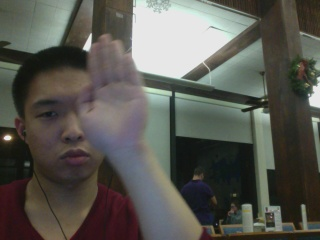
\includegraphics[width=40px, height=30px]{../data/analysis/img0013.jpg}
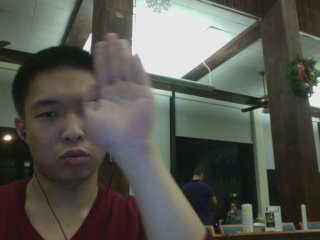
\includegraphics[width=40px, height=30px]{../data/analysis/img0014.jpg}
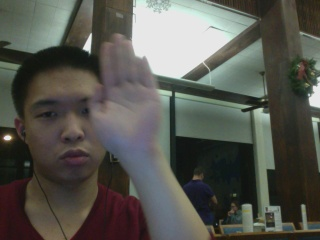
\includegraphics[width=40px, height=30px]{../data/analysis/img0015.jpg}
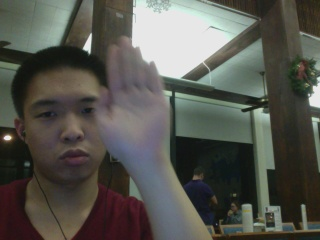
\includegraphics[width=40px, height=30px]{../data/analysis/img0016.jpg}
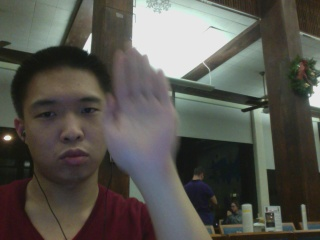
\includegraphics[width=40px, height=30px]{../data/analysis/img0017.jpg}
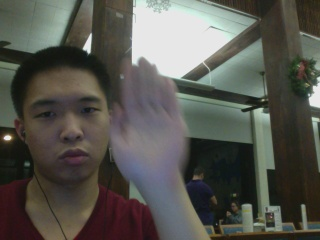
\includegraphics[width=40px, height=30px]{../data/analysis/img0018.jpg}
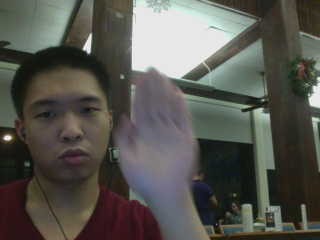
\includegraphics[width=40px, height=30px]{../data/analysis/img0019.jpg} \\
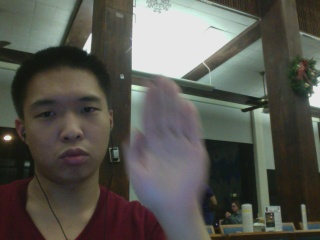
\includegraphics[width=40px, height=30px]{../data/analysis/img0020.jpg}
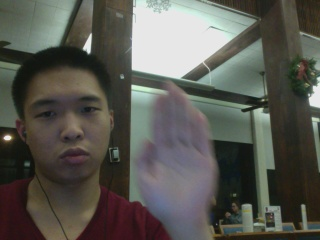
\includegraphics[width=40px, height=30px]{../data/analysis/img0021.jpg}
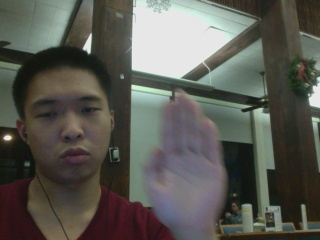
\includegraphics[width=40px, height=30px]{../data/analysis/img0022.jpg}
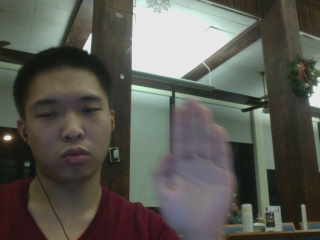
\includegraphics[width=40px, height=30px]{../data/analysis/img0023.jpg}
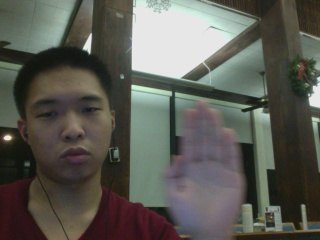
\includegraphics[width=40px, height=30px]{../data/analysis/img0024.jpg}
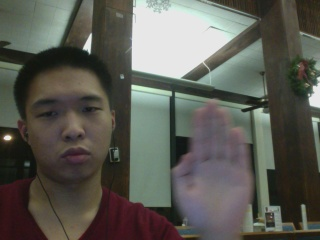
\includegraphics[width=40px, height=30px]{../data/analysis/img0025.jpg}
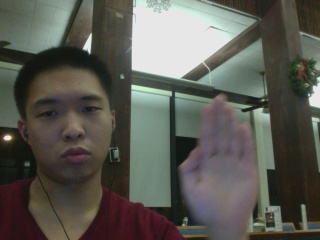
\includegraphics[width=40px, height=30px]{../data/analysis/img0026.jpg}
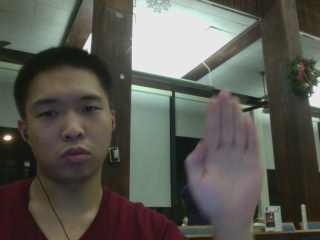
\includegraphics[width=40px, height=30px]{../data/analysis/img0027.jpg}
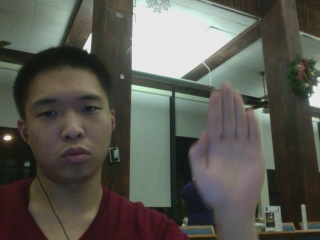
\includegraphics[width=40px, height=30px]{../data/analysis/img0028.jpg}
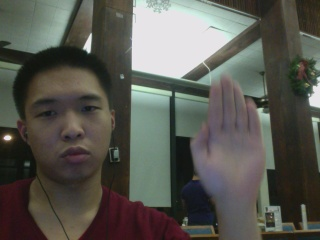
\includegraphics[width=40px, height=30px]{../data/analysis/img0029.jpg} \\
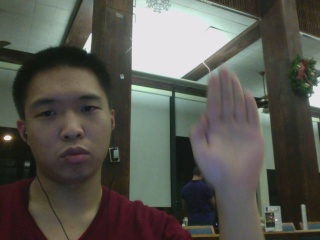
\includegraphics[width=40px, height=30px]{../data/analysis/img0030.jpg}
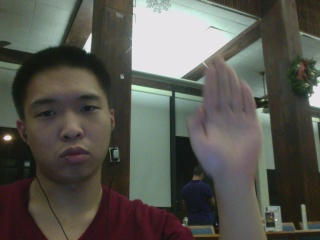
\includegraphics[width=40px, height=30px]{../data/analysis/img0031.jpg}
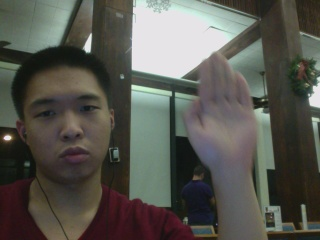
\includegraphics[width=40px, height=30px]{../data/analysis/img0032.jpg}
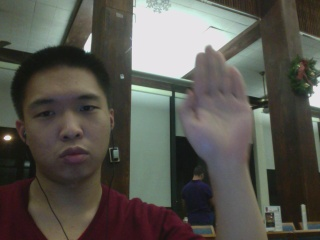
\includegraphics[width=40px, height=30px]{../data/analysis/img0033.jpg}
\includegraphics[width=40px, height=30px]{../data/analysis/img0034.jpg}
\includegraphics[width=40px, height=30px]{../data/analysis/img0035.jpg}
\includegraphics[width=40px, height=30px]{../data/analysis/img0036.jpg}
\includegraphics[width=40px, height=30px]{../data/analysis/img0037.jpg}
\includegraphics[width=40px, height=30px]{../data/analysis/img0038.jpg}
\includegraphics[width=40px, height=30px]{../data/analysis/img0039.jpg} \\
\includegraphics[width=40px, height=30px]{../data/analysis/img0040.jpg}
\includegraphics[width=40px, height=30px]{../data/analysis/img0041.jpg}
\includegraphics[width=40px, height=30px]{../data/analysis/img0042.jpg}
\includegraphics[width=40px, height=30px]{../data/analysis/img0043.jpg}
\includegraphics[width=40px, height=30px]{../data/analysis/img0044.jpg}
\includegraphics[width=40px, height=30px]{../data/analysis/img0045.jpg}
\includegraphics[width=40px, height=30px]{../data/analysis/img0046.jpg}
\includegraphics[width=40px, height=30px]{../data/analysis/img0047.jpg}
\includegraphics[width=40px, height=30px]{../data/analysis/img0048.jpg}
\includegraphics[width=40px, height=30px]{../data/analysis/img0049.jpg}
\caption{The 50 frame sequence we used to test the components of our pipeline.}
\label{seq-original}
\end{figure}

To gauge the various components of our pipeline, we created a 50-frame sequence, shown in Figure \ref{seq-original}. We created 8 pipelines, generated by our choices of whether to remove faces, apply background subtraction, and use a Kalman filter. We always perform optical flow to measure the direction of the hand. After generating the images, we went through the images by hand to count the number of true and false positives. We define a true positive when we have a green box around the hand, and we define a false positive whenever we see a yellow or a green box surrounding something that is not a hand. See Table \ref{datatable} for our results, and see the \texttt{data} subdirectories for the annotated images for each pipeline.

\noindent
\begin{figure}[H]
\begin{center}
\begin{tabular}{|c|c|c|c|c|c|c|c|c|c|}
\hline
\shortstack{Pipeline \\ Type} &		FPS &	\shortstack{True \\ Pos.} &	TPR &		\shortstack{False \\ Pos. }&	 FPR &		\shortstack{Average \\ $v_x$} & 	\shortstack{Average \\ $v_y$} & 	\shortstack{Average \\ Width} &	\shortstack{Average \\Height} \\	\hline \hline
None    & 	25.348	  & 	46		        &	0.939     &		35                        &	0.714     &		-18.772 &	20.701 &	73.061 &	131.389	\\ \hline
Face &	13.373 &	33 &	0.673 &	0 &	0 &	-17.565 &	28.768	& 49.429	& 88.837 \\ \hline
Kalman &	22.841 &	45	&0.918	&4	&0.0816&	-31.605	&30.921	&61.735&	110.878		\\ \hline
BG	 & 21.478&	37	&0.755	&32	&0.653	&-16.85	&-7.266	&76.551	&137.571		\\ \hline
\shortstack{Face, \\ Kalman}	&11.795&	32	&0.653&	0	&0&	-28.157	&46.57	&42.429&	76.163	\\ \hline
\shortstack{Face, BG}	&12.423&	31	&0.633&	2	&0.0408&	-15.287&	16.235&	51.49&	92.571		\\ \hline
\shortstack{BG, \\ Kalman}&	19.841&	23&	0.469	&25	&0.510	&-0.476	&-5.81	&66.265&	118.89	\\ \hline
All	&10.888&	28	&0.571&	0	&0	&-11.663&	24.01&	46.122	&82.939 \\
\hline
\end{tabular}
\end{center}
\caption{Results of running all the combinations of components in our pipeline on the same 50 frame sequence.}
\label{datatable}
\end{figure}

Applying our hand detector alone had a very high true positive rate, but also generated many false positives as one would guess. We note that performing face removal using OpenCV's frontal face Haar cascade significantly decreases the frame rate in all cases (and hence, slower performance), but dramatically decreases the number of false positives. 

We note that a background subtractor generates many false positives when applied alone and with a Kalman filter. Furthermore, we noted that using background subtraction does not detect a hand if the hand stays perfectly still--overtime, the hand will blend into the background and will not be seen by our detector. 

A Kalman filter generates the fewest false positives for the number of true positives it detected, and when combined with face removal, generates no false positives. Combining all three of these components generates no false positives, but detects fewer true positives than only applying face removal and using a Kalman filter. 

Hence, if our main priority is to eliminate false positives, then we only need to apply face removal and use a Kalman filter. If our main priority is to generate as many true positives while maintaining a fairly low false positive rate, then we should only use Kalman filter. For our maps application running on a medium sized EC2 instance \cite{ec2}, we discovered that running the entire pipeline was too slow to be usable, and that running only the face removal and Kalman filter components made the application much faster and a lot more responsive to user movement.

We note the wide discrepancies in average velocity and average hand size. Thus, the components we use in our pipeline dramatically affects the resulting output in the maps application.


\section{Conclusion}

In this paper, we provided a method to quickly train a hand detector using only a few images, and achieved comparable hand tracking accuracy to using a perfect hand detector. We also described and built a system for running our pipeline on a real time application in which the user controls Google Maps by moving one's hand. For future work, we would like to explore how to generalize this process. 

We would like to explore how well this pipeline works for different kinds of hand positions, e.g. fists, detecting certain digit configurations, and more. Furthermore, we would like to explore other components that can be added to our pipeline to further decrease the number of false positives and increase the number of true positives, while maintaining a relatively high frame rate to actually be usable in applications. A limitation of this current pipeline, however, is that only one hand can be tracked. It becomes unclear how to generalize some of the components of our current pipeline when we attempt to track multiple hands in the frame, e.g. it is unclear how many Kalman prediction windows to use and how we use these multiple windows.

Thus, by using less training data and a bit more computation power, we hope that commodity webcams will one day be able to emulate many of the features offered in a Kinect.

\section{Appendix}

\appendix
\section{Source Code}
\label{sourcecode}
To checkout the source vode, visit \url{https://github.com/kennyyu/cs283-project}. See the \texttt{README} for information on how to run the various pipelines, the server, and analyzer scripts. The generated cascades are located in the \texttt{cascades} directory, and the images we used to train our detector are located in the \texttt{data/positives} directory.

\section{Maps Application}
\label{mapsapp}
To view the live running maps application, visit \url{http://goo.gl/pcNxG}. You must use Chrome, have enabled web sockets (see \texttt{chrome://flags}), and have a connected webcam. The application is currently running on a medium Amazon EC2 instance \cite{ec2}.

\begin{thebibliography}{99}

\bibitem{ec2}
Amazon Elastic Compute Cloud. \textless\url{http://aws.amazon.com/ec2/}\textgreater.

\bibitem{cascadetutorial}
  ``Cascade Classifier Training''. OpenCV 2.4.9 Documentation. Accessed 12 Dec. 2012. \textless\url{http://docs.opencv.org/trunk/doc/user_guide/ug_traincascade.html}\textgreater.

\bibitem{webtutorial}
Dirksen, Joe. ``Face detection using HTML5, javascript, webrtc, websockets, Jetty, and OpenCV''. Smartjava.org. 19 Apr. 2012. \textless\url{http://www.smartjava.org/content/face-detection-using-html5-javascript-webrtc-websockets-jetty-and-javacvopencv}\textgreater.

\bibitem{googlemaps}
Google Maps. Google, Inc. \textless\url{http://maps.google.com}\textgreater.

\bibitem{lucaskanade}
Lucas, Bruce D. and Takeo Kanade. ``An Iterative Image Registration Technique with an Application to Stereo Vision''. Proceedings of Imaging Understanding Workshop, 1981, pp. 121-1380. 

\bibitem{opencv}
OpenCV 2.4.1. \textless\url{http://opencv.org/}\textgreater.

\bibitem{tornado}
Tornado Web Server 2.4.1. \textless\url{http://www.tornadoweb.org/}\textgreater.

\bibitem{negatives}
Seo, Naotoshi. ``Tutorial: OpenCV haartraining''. \textless\url{http://note.sonots.com/SciSoftware/haartraining.htm}\textgreater.

\bibitem{violajones}
Viola, Paul and Michael Jones. ``Rapid Object Detection using a Boosted Cascade of Simple Features''. Conference on Computer Vision and Pattern Recognition (CVPR), 2001, pp. 511-518. 

\bibitem{webrtc}
``Web Real-Time Communications Working Group Charter''. W3C. 4 Dec, 2012. \textless\url{http://www.w3.org/2011/04/webrtc-charter.html}\textgreater.

\bibitem{websockets}
``The WebSocket API''. W3C. 4 Dec, 2012. \textless\url{http://dev.w3.org/html5/websockets/}\textgreater.

\bibitem{kalmanfilter}
Welch, Greg and Gray Bishop. \emph{An Introduction to the Kalman Filter}. University of North Carolina at Chapel Hill. SigGraph 2001. Ch. 4. pp. 19-29. \textless\url{http://www.cs.unc.edu/~tracker/media/pdf/SIGGRAPH2001_CoursePack_08.pdf}\textgreater.

\end{thebibliography}

\end{document}